\documentclass[mathNotesPreamble]{subfiles}
\begin{document}
%\relscale{1.4} %TODO
\section{15.4: The Chain Rule}

  \noindent
  \fbox{\parbox{0.9875\linewidth}{
    \textbf{Theorem 15.7: Chain Rule (One Independent Variable)}\\
    Let $z$ be a differentiable function of $x$ and $y$ on its domain, where $x$ and $y$ are differentiable functions of $t$ on an interval $I$. Then
      \[\frac{dz}{dt}=\frac{\partial z}{\partial x}\frac{dx}{dt}+\frac{\partial z}{\partial y}\frac{dy}{dt}.\]
  }}
  \vspace*{\baselineskip}

  \noindent
  \begin{minipage}{0.65\linewidth}
  \textit{Note:} 
    \begin{itemize}
      \item For $z=f\parens{x(t), y(t)}$, $z$ is the dependent variable, $t$ is the independent variable, and $x$ and $y$ are \newline\textbf{intermediate variables}.
      \item Since $x$ and $y$ only depend on $t$, we use the `ordinary' derivative symbol
      \item Theorem 15.7 generalizes to functions of $n$ variables
    \end{itemize}
  \end{minipage}%
  \begin{minipage}{0.35\linewidth}
    \begin{flushright}
      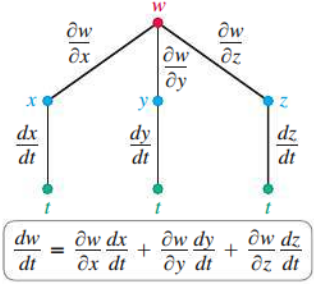
\includegraphics[width=0.9\linewidth]{images/briggs_15_04/fig15_37}
    \end{flushright}
  \end{minipage}
  \vspace*{\baselineskip}

  \begin{ex*}
    Find the derivative of the following functions using the chain rule where appropriate.
  \end{ex*}
  \begin{tasks}[after-item-skip=\stretch{1}, label=](1)
    \task $z=x^2-2y^2+20$ where $x=2\cos(t)$ and $y=2\sin(t)$
  \end{tasks}
  \vspace*{\stretch{1}}
  \pagebreak
  \begin{tasks}[after-item-skip=\stretch{1}, label=, resume](1)
    \task $w=\sin(12x)\cos(2y)$ where $x=t/2$ and $y=t^3$
    \task $Q=\sqrt{3x^2+3y^2+2z^2}$ where $x=\sin(t)$, $y=\cos(t)$, and $z=\cos(t)$.
  \end{tasks}
  \vspace*{\stretch{1}}
  \pagebreak

  \noindent
  \fbox{\parbox{0.9875\linewidth}{
    \textbf{Theorem 15.8: Chain Rule (Two Independent Variables)}\\
    Let $z$ be a differentiable function of $x$ and $y$, where $x$ and $y$ are differentiable functions of $s$ and $t$. Then
      \[\frac{\partial z}{\partial s}=\frac{\partial z}{\partial x}\frac{\partial x}{\partial s}+\frac{\partial z}{\partial y}\frac{\partial y}{\partial s} \quad\textnormal{and}\quad \frac{\partial z}{\partial t}=\frac{\partial z}{\partial x}\frac{\partial x}{\partial t}+\frac{\partial z}{\partial y}\frac{\partial y}{\partial t}.\]
  }}
  \begin{center}
    \hspace*{\stretch{1}}
    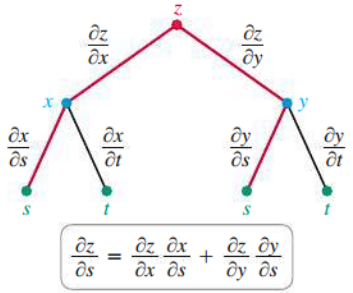
\includegraphics[width=0.315\linewidth]{images/briggs_15_04/fig15_39}
    \hspace*{\stretch{1}}
    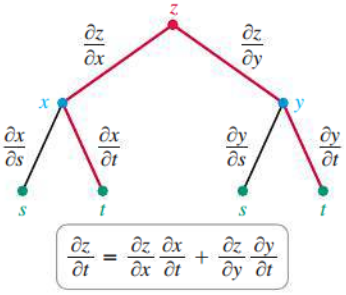
\includegraphics[width=0.315\linewidth, trim={0mm 1.0mm 0mm 0mm},clip]{images/briggs_15_04/fig15_40}
    \hspace*{\stretch{1}}
  \end{center}

  \begin{ex*}
    For $z=e^{5x+8y}$, where $x=7st$ and $y=5s+t$, find $z_s$ and $z_t$.
  \end{ex*}
  \vspace*{\stretch{1}}
  \pagebreak

  \begin{ex*}
    For $z=\sin(2x)\cos(3y)$, where $x=s+t$ and $y=s-t$, find $\partial z/\partial s$ and $\partial z/\partial t$.
  \end{ex*}
  \vspace*{\stretch{1}}

  \begin{ex*}
    For $r=\ln(x^2+xy+y^2)$, where $x=2st$ and $y=s/t$, find $\partial r/\partial s$ and $\partial r/\partial t$.
  \end{ex*}
  \vspace*{\stretch{1}}

  \pagebreak

  \noindent
  \fbox{\parbox{0.9875\linewidth}{
    \textbf{Theorem 15.9: Implicit Differentiation}\\
    Let $F$ be differentiable on its domain and suppose $F(x,y)=0$ defines $y$ as a differentiable function of $x$. Provided $F_y\neq 0$,
      \[\frac{dy}{dx}=-\frac{F_x}{F_y}.\]
  }}
  
  \textit{Note}: The above derivation comes from using the chain rule on $F(x,y)=0$.
  \vspace*{2\baselineskip}
  \begin{ex*}
    For $4x^3+2x^2y-3y^3=0$, find $\dydx$ implicitly.
  \end{ex*}
  \vspace*{\stretch{1}}
  \begin{ex*}
    For $xy+xz+5yz=42$, find $\partial z/\partial x$ and $\partial z/\partial y$ implicitly.
  \end{ex*}
  \vspace*{\stretch{1}}
  \pagebreak

  \begin{ex*}
    For $xyz+2yz+3xz=4x+2y-3z$, find $\partial z/\partial x$ and $\partial z/\partial y$.
  \end{ex*}
  \vspace*{\stretch{1}}

  \begin{ex*}
    Consider the surface $z=f(x,y)=3x^2+9y^2+4$ and the curve $C$ given parametrically by $x=\cos(t)$ and $y=\sin(t)$ where $0\leq t\leq 2\pi$. Find $z'(t)$ and find $t$ such that $z'(t)>0$.
  \end{ex*}
  \vspace*{\stretch{1}}

  \pagebreak
  
\end{document}